\chapter{Lead Management}

Lead Management is one part of the customer acquisition process. This process follows several phases, which is referred by multiple authors as the \textbf{Sales Funnel} or \textbf{Conversion Funnel}. 
While comparing different literature, it soon becomes clear that there is no exact definition of ``Lead Management'' \cite{Vossebein2024LeadManagement, WengerLeadmanagement2021}.

In 2024, \citeauthor{Vossebein2024LeadManagement} define a lead as 

\begin{quote}
\textit{``a potential new customer who expresses interest in a company's product or service by voluntarily providing their contact information. This may refer to either an individual or a company.''} \cite{Vossebein2024LeadManagement}
\end{quote} 

Lead Management describes the processes involved while generating, qualifying and conversion of leads into real sales. It cannot be bound to a specific department, however mostly sales and marketing areas are involved during Lead Management \cite{Vossebein2024LeadManagement}.   
Historically, sales and marketing departments were working alongside each other, but did not combine their forces. For example, \citeauthor{WengerLeadmanagement2021} mentions that during a crisis, marketing will blame sales that they do not utilize their great marketing campaigns. Sales will say that marketing did not understand the customer and the campaign was aiming for the wrong target group \cite{WengerLeadmanagement2021}. This old-fashioned view changed dramatically during the COVID-19. Since then, digital marketing budget was increased by a large amount across industries and has reached $54\%$ of total marketing budget in 2022 \cite{Vossebein2024LeadManagement}. This trend is reinforced by the growing influence of Generation Z, born between 1990 and 2010, who are now increasingly entering management positions and, having grown up with the internet and social networks, actively driving the shift towards digital and data-driven marketing strategies \cite{Vossebein2024LeadManagement, WengerLeadmanagement2021}.

\newpage

This growing interest in digital marketing goes along with the general concept of the so-called \textbf{Funnel Concept}. The funnel concept can be applied to both marketing and sales processes and displays the process of (digital) customer or sales acquisition \cite{Steuernagel2021, Vossebein2024LeadManagement}. Both in Sales and Lead management, the funnel shape is supposed to represent the decreasing amount of total leads from phase to phase \cite{Vossebein2024LeadManagement}. First of all, we will focus on the \textbf{Sales Funnel}, which can be seen in Figure \ref{fig:sales_funnel}. 


\section{Sales Funnel}
\label{sec:sales_funnel}

The Sales Funnel, often called the \ac{aida} model, is a four step process with stages \textit{Awareness}, \textit{Interest}, \textit{Desire} and \textit{Action}. The Sales Funnel is traditionally managed by marketing departments \cite{Steuernagel2021}.

At the top of the funnel lies the \textbf{Awareness} phase, which represents the initial point of contact between a potential customer and a company’s products. In this stage, the marketer’s primary objective is to capture attention and ensure that the prospect becomes aware of both their own problem and the company’s potential solution. As \citeauthor{SapianVyshnevska2019} point out, awareness relies on three fundamental aspects: the prospect must understand \textit{that} the company exists, \textit{what} it offers, and \textit{why} it might be relevant to them \cite{SapianVyshnevska2019}.To achieve this, organizations employ a broad range of communication channels, many of which operate in highly competitive and fast-paced environments. Traditional advertising, social media campaigns, blog posts, ads, webinars and mail all contribute to increasing visibility and ensuring the brand is presented alongside other offers. In today’s digital ecosystem, awareness is often generated not only through marketing actions but also through indirect influences such as  journalists, influencers, and user-generated content \cite{SapianVyshnevska2019, Steuernagel2021}.

\newpage

Afterwards, customers develop an \textbf{Interest} in the product, start performing research and feel a desire to purchase the product. As consumers gather more information, they begin to formulate reasons for choosing a company’s product or service. This creates an important window of opportunity for building a relationship and nurturing the emerging lead \cite{Steuernagel2021}. Methods of binding the customer towards a company can be customer guides, online videos, media interviews, blogs, and even well-trained customer service interactions \cite{SapianVyshnevska2019}. 

The transition from interest to \textbf{Desire} is not strictly linear. As \citeauthor{SapianVyshnevska2019} point out, the desire stage can vary significantly in duration depending on the industry, as customers often spend longer periods thinking about alternatives, comparing offers, and reassuring before committing to a product \cite{SapianVyshnevska2019}. In digital contexts, factors such as transparent shipping policies, clear return procedures, security guarantees, or authentic customer reviews play a role in increasing or weakening the intent. The \textit{recognition of need} is mainly build through the digital marketing methods mentioned above \cite{Steuernagel2021, Vossebein2024LeadManagement}.

To satisfy that desire, the prospect takes \textbf{Action}. However, every prospect is different and it takes a different time span until a prospect will become a customer. To streamline this experience, it is important to make the buying process as easy as possible, that the potential customer does not get distracted \cite{SapianVyshnevska2019}.
That is the starting point for the \textbf{Lead Funnel} \cite{WengerLeadmanagement2021}.

\begin{figure}
    \centering
    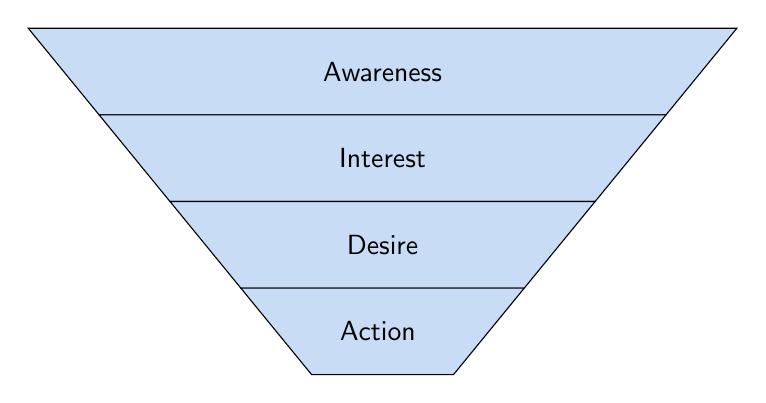
\begin{tikzpicture}[font=\sffamily, align=center]

        % Farben
        \definecolor{lightblue}{RGB}{200,220,245}

        % Trichter (invers)
        \def\levels{
            {Awareness},
            {Interest},
            {Desire},
            {Action}
        }
        % Maße
        \def\width{9}    % obere Breite
        \def\height{1.1} % Höhe jeder Ebene
        \def\num{4}      % Anzahl der Ebenen

        % Zeichne den invertierten Trichter
        \foreach \i [count=\n from 0] in \levels {
            \pgfmathsetmacro{\topwidth}{\width*(1 - (\n)/(\num+1))}
            \pgfmathsetmacro{\bottomwidth}{\width*(1 - (\n+1)/(\num+1))}
            \pgfmathsetmacro{\yshift}{-\n*\height}
            \draw[fill=lightblue, draw=black] 
                (-\topwidth/2, \yshift) -- (\topwidth/2, \yshift)
                -- (\bottomwidth/2, \yshift - \height) -- (-\bottomwidth/2, \yshift - \height)
                -- cycle;
            \node at (0, \yshift - 0.5*\height) {\i};
        }

    \end{tikzpicture}

    \caption{Sales Funnel \cite{Steuernagel2021, WengerLeadmanagement2021}}
    \label{fig:sales_funnel}
    
\end{figure}



\section{Lead Funnel}

\begin{figure}
    \centering
    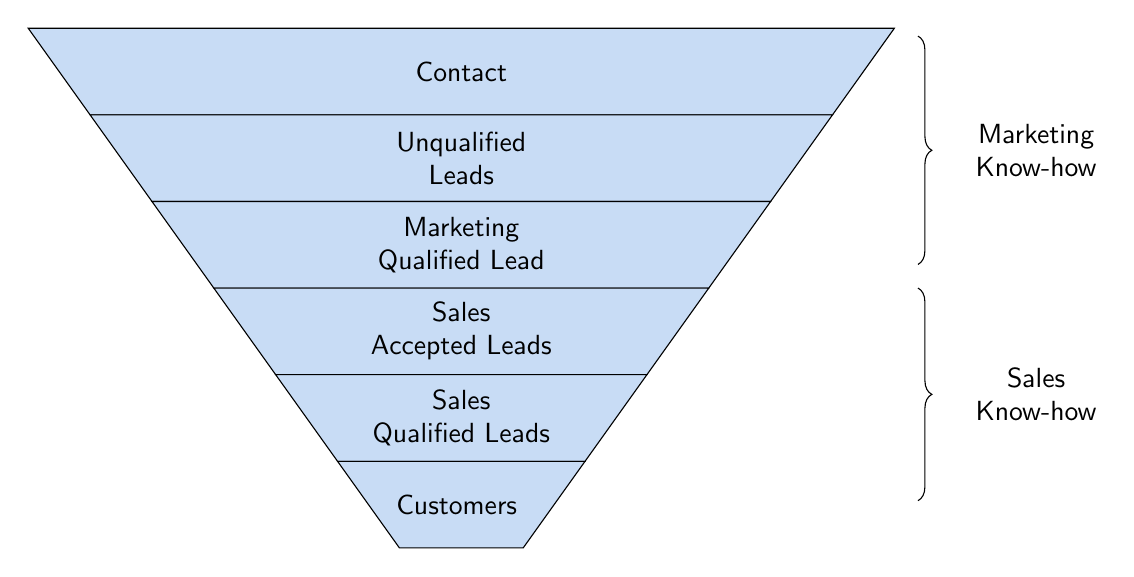
\begin{tikzpicture}[font=\sffamily, align=center]

        % Farben
        \definecolor{lightblue}{RGB}{200,220,245}

        % Trichter (invers)
        \def\levels{
            {Contact},
            {Unqualified\\Leads},
            {Marketing\\Qualified Lead},
            {Sales\\Accepted Leads},
            {Sales\\Qualified Leads},
            {Customers}
        }

        % Maße
        \def\width{11}    % obere Breite
        \def\height{1.1} % Höhe jeder Ebene
        \def\num{6}      % Anzahl der Ebenen

        % Zeichne den invertierten Trichter
        \foreach \i [count=\n from 0] in \levels {
            \pgfmathsetmacro{\topwidth}{\width*(1 - (\n)/(\num+1))}
            \pgfmathsetmacro{\bottomwidth}{\width*(1 - (\n+1)/(\num+1))}
            \pgfmathsetmacro{\yshift}{-\n*\height}
            \draw[fill=lightblue, draw=black] 
                (-\topwidth/2, \yshift) -- (\topwidth/2, \yshift)
                -- (\bottomwidth/2, \yshift - \height) -- (-\bottomwidth/2, \yshift - \height)
                -- cycle;
            \node at (0, \yshift - 0.5*\height) {\i};
        }

        % Klammern und Beschriftung rechts
        \draw [decorate, decoration={brace, amplitude=5pt}] 
            (5.8, -0.1) -- (5.8, -3.0) node[midway, xshift=1.5cm, align=center]{Marketing\\Know-how};

        \draw [decorate, decoration={brace, amplitude=5pt}] 
            (5.8, -3.3) -- (5.8, -6.0) node[midway, xshift=1.5cm, align=center]{Sales\\Know-how};

        
    \end{tikzpicture}

    \caption{Lead funnel \cite{WengerLeadmanagement2021}}
    \label{fig:lead_funnel}
\end{figure}

After the potential customer went through the \ac{aida} model and is ready to perform action (e.g. placing an offer, visiting a website, making a call), his journey continues with the Lead Funnel.
The first three steps are mostly managed by marketing departments and their success relies on Marketing Know-how (cf. figure \ref{fig:lead_funnel}) \cite{Steuernagel2021}. The first one of these is a phase called \textbf{Contact}. Here the potential customer gets in first contact with the company, e.g. though filling out a form on a website. 

Directly afterwards, the \textbf{Unqualified Lead} is created. The task of the marketing department is now to gather as much information as possible and decide whether the individual fits the general target profile. The goal of this phase is therefore to enrich the contact with basic demographic and company-related data that allows for an initial qualification \cite{Steuernagel2021, WengerLeadmanagement2021}.

Once these criteria are met, the prospect evolves into a \textbf{Marketing Qualified Lead}. While much of the early-stage qualification is driven by digital marketing automation, meaningful qualification increasingly requires human interaction as prospects move closer to a potential purchase \cite{Steuernagel2021}. Marketing typically decides whether the lead operates within the relevant target group that is supposed to be addressed. These insights are important information before a lead can be handed over to the sales department. 

If all criteria is met, the next stage, \textbf{Sales Accepted Lead}, marks the point where the sales team formally acknowledges the lead as relevant and takes the next actions. From that point on, the success relies on Sales Know-how \cite{WengerLeadmanagement2021}.

Historically, frameworks such as \ac{bant} were used to reach the \textbf{Sales Qualified Lead} state, whereas today more sophisticated methodologies like \ac{meddic} or \ac{champ} help sales teams evaluate opportunities in a structured and data-driven manner.

At the very end of the funnel, the prospect turns into a real \textbf{customer}. With that, the lead management process ends. Yet, the customer contact should not suddenly stop. Literature describes several customer retention programs to boost customer loyalty after the first initial sale \cite{Steuernagel2021}. However, they are not part of this project paper.


\section{Performance Metrics}
\label{sec:performance-metrics}

This section introduces the most important \ac{kpi}s inside Lead Management. In general, literature differentiates between metrics built for \textbf{lead scoring}, answering the question \textit{"how good is this lead?"} and \textbf{process performance metrics} designed for rating the lead management itself to answer the question \textit{"how good is the lead management?"} \cite{pedowitz2025kpis, Wu2024lead_scoring}.

In 2023, \citeauthor{Wu2024lead_scoring} performed a systematic literature review on the state of lead scoring metrics.
Their review spans 44 academic and industrial studies and identifies traditional scoring mechanisms but also modern data-driven predictive models. The authors highlight that predictive lead scoring approaches, such as decision trees and random forests, consistently outperform traditional techniques in terms of sales performance outcomes. Traditional techniques include \ac{kpi}s such as conversion rates, profitability, and cost efficiency \cite{Wu2024lead_scoring}. 

Among the process metrics, lead conversion rate emerges as the most frequently used performance measurement, followed by cost reduction, number of qualified leads and annual revenue \cite{Wu2024lead_scoring}. 

Some of \citeauthor{Wu2024lead_scoring}s mentioned \ac{kpi}s are presented in table \ref{sec:performance-metrics}. They will be used in chapter four to analyze the case study at Bosch.

\begin{table}
\centering
\renewcommand{\arraystretch}{1.3}

\begin{tabular}{p{2.5cm} | p{5.5cm} | >{$}c<{$}}

\textbf{Metric} & \textbf{Meaning} & \textbf{Formula} \\
\hline
Lead Cycle Time &
Time from lead creation until qualification or final closure. &
Date_{Closure} - Date_{Creation} \\
\hline
Time-to-First-Touch &
Time until first contact by Marketing or Sales after lead creation. &
Date_{FirstContact} - Date_{Creation} \\
\hline
Throughput Rate &
Number of leads processed in a defined time period. &
\frac{Total Leads Processed}{Time Period} \\
\hline
Conversion Rate &
Percentage of leads that move from one funnel stage to the next.
 &
\frac{Leads in Next Stage}{Leads in Current Stage} \times 100 \\
\hline
Lead Leakage Rate &
Proportion of leads dropping out between two stages. &
\frac{Leads Lost}{Leads Entering Stage} \times 100 \\
\hline
Sales Cycle Duration &
Average duration from SQL qualification to closed deal.
 &
Date_{Closure} - Date_{Qualification} \\
\hline
Cost per Lead &
Marketing and sales spend divided by the number of leads.
&
\frac{Total Marketing + Sales Cost}{Number of Leads} \\
\hline
Cost per Order &
Total cost per successfully closed sale.
 &
\frac{Total Marketing + Sales Cost}{Number of Closed Deals} \\
\end{tabular}

\caption{Lead Management Process KPIs \cite{pedowitz2025kpis, haufe2018vierkpis}}
\label{tab:lead_process_kpis}
\end{table}

In general, Lead Management is very rarely connected with Data Mining, not even speaking of Process Mining.  In one of \citeauthor{LeadmanagementDataMining2021} paper's called \textit{``Lead management optimization using data mining: A case in the telecommunications sector''} from 2021, they cite that only nine different papers existed on the relationship between lead management and data mining. In 2025, not much has changed in the perspective of Process Mining. A search for the string \textit{``process mining lead management''} even returns zero matching articles on Google Scholar. This indicates the research that still has to be performed on this topic \cite{LeadmanagementDataMining2021}.